%%%%%%%%%%%%%%%%%%%%%%% Grundeinstellungen %%%%%%%%%%%%%%%%%%%%%%%%%%%
% 'Artikel' Dokumentenklasse und Standardschriftgröße  
\documentclass[12pt]{scrartcl}

% Setzt das Papierformat und den Rand auf 2.5cm                                                      
\usepackage[paper=a4paper,left=2.5cm,right=2.5cm,top=2.5cm,bottom=2.5cm]{geometry}  

% Setzt die Einrückung von Absätzen auf gegebenen Abstand
%\setlength{\parindent}{0mm}

% Legt Zeilenabstand fest                                                         
\usepackage[onehalfspacing]{setspace}                                               

% Legt Zeichenkodierung fest                                                            
\usepackage[utf8]{inputenc}                                                         

% Neue Deutsche Rechtschreibung
\usepackage[ngerman]{babel}  

% Legt FontKodierung fest
\usepackage[T1]{fontenc}

% Versieht Referenzen mit Bezeichnung des Objektes                                                      
%\usepackage[ngerman]{varioref}   

% Empfohlener T1-Font für deutsche Texte                                               
\usepackage{lmodern} 

% Deutsche Zitate mit \enqoute{},\enqoute*{} 
\usepackage[babel,german=quotes]{csquotes}

%Einstellungen für Bibliographien mit "biber"                                                              
\usepackage[backend=biber, style=numeric-verb,sorting=none]{biblatex}

%%%%%%%%%%%%%%%%%%%% Seitenlayout %%%%%%%%%%%%%%%%%%%%%%%%%%%%%%%%%%%%

% Ermöglicht detailierte Bearbeitung der Kopf- und Fußzeile
\usepackage{fancyhdr} 

% Setzt Kopf und Fußzeile zurück                                                              
\fancyhf{} 	     
         
% Höhe der Kopfzeile                                                          
\setlength{\headheight}{28.0pt}   

% Höhe der Fußzeile                                                  
\setlength{\footskip}{18.0pt}                                                      

% Dicke des Kopfzeilentrennstrichs
\renewcommand{\headrulewidth}{.5 pt}     

% Dicke des Fußzeilentrennstrichs                                     
\renewcommand{\footrulewidth}{.5 pt}                                                 

%Test ob Variable gesetzt ist oder nicht
%\ifdefined\EN% 
	% Angabe Links-Oben
%\lhead{\textbf{\EN}}
%\else%
%    \lhead{\textbf{\textcolor{red}{VERSUCHNAME!!!}}}
%\fi%      
                                                            
% Angabe Mitte-Oben
%\chead{}  
\lhead{\textbf{Beobacher und Bewusstsein}\\Joshua Luckey}
% Angabe Rechts-Oben                                                                         
\rhead{Seminar: Quantenmechanik  und\\ Messprozess (Prof. H. Päs)}  

% Angabe Links-Unten                                                                    
%\lfoot{}        

% Angabe Mitte-Unten                                                                   
\cfoot{\textbf{\thepage\ von \pageref{LastPage}}}  

% Angabe Rechts-Unten                                 
\rfoot{}                                           

% Anwenden des erweiterten Seitenlayouts
\pagestyle{fancy}      

                                                              
%%%%%%%%%%%%%%%%%%%%%%%% MINT %%%%%%%%%%%%%%%%%%%%%%%%%%%%%%%%%%%%%%%%
% Fügt mathematische Symbole hinzu, setzt Grenzen, Limiten und Indizes unter das Symbol und nicht dahinter
\usepackage[sumlimits,intlimits,namelimits]{amsmath}  

% Fügt Symbole wie z.B. Zahlenmengen wie $\mathbb{R}$ hinzu                             
\usepackage{amssymb}    
                                                             
% Beweißumgebung
\usepackage{amsthm}  

% Font für Mathematikumgebung                                                              
\usepackage{amsfonts}    
                                                          
% Verbesserte Gleichungsumgebung mit \begin{empheq}[<Aussehen>]{<Umgebungstyp>} ... \end{empheq}
\usepackage{empheq}      

% Ergänzungen für physikalische Arbeiten
\usepackage{physics}

% Chemische Struktur und Summenformeln mit \ce{<Summenformel>}                                                          
%\usepackage[version=3]{mhchem}  

% Chemische Valenzstrichformeln für ganze Moleküle mit\chemfig{<Molekül-Aufbau>}                                                   
%\usepackage{chemfig}                                                               

% Verbesserte Formatierung von größen mit Einheiten 
\usepackage{siunitx}                                                               
	% 'Mal'-Zeichen auf \cdot und Dezimaltrennzeichen auf ',' 
	\sisetup{locale = DE,prefixes-as-symbols = true}                                   
                                                                            
	% Vereinfachtes eintragen von Unsicherheiten mit '42.6(4)' --> '42.6 +/- 0.4'          
	\sisetup{separate-uncertainty=true} 
	
	\sisetup{per-mode=reciprocal}                                                                                                                   

 
                                                            
% Fügt verbesserte Vektorpfeile hinzu \vv{<Vektorname>} 
\usepackage[b]{esvect}  

% Brüche mit "/" im Text mit \sfrac{}                                                            
\usepackage{xfrac}

% Darstellung von 2D Feldern 
\usepackage{array}

% Differentialoperatoren,-quotienten und Klammern mit \od[]{}{}, \pd[]{}{}, \del{}, \sbr{}, \cbr{}
\usepackage{commath}

% Pseudocode-Umgebungen 																
\usepackage{algorithmicx}
\usepackage{algpseudocode}

% Einbinden von SourceCode Dateien (listing)
\usepackage{listings}
	% Auswählen der Programmiersprache
	\lstset{language=Python}

%%%%%%%%%%%%%%%%% Seiten- und Floateinstellungen %%%%%%%%%%%%%%%%%%%%%
% Einbinden von Grafiken mit '\includeudegraphics[<Optionen>]{<Grafikpfad>}' und Veränderungen im Text, wie z.B. Schriftfarbe 
\usepackage{graphicx} 

% Fügt Möglichkeit für textumflossende Grafiken und Tabellen hinzu \begin{floating<figure/table>}[option]{width} ... \caption ... \end{floatingfigure}                                                              
\usepackage{floatflt}        
\usepackage{wrapfig}

% Ermöglicht das Hinzufügen von Unterabbildung zu einer Abbildung                                                 
\usepackage{subfig} 
%\usepackage{subfigure} 
%\usepackage{subcaption}

% Verhindert das Wandern von "floating" Umgebungen über eine Bestimmte Grenze (hier: Sections) oder mit \FloatBarrier                                                             
\usepackage[section]{placeins}

% Ermöglicht Zeichnungen im Dokument \begin{tikzpicture} ... \end{tikzpicture}
\usepackage{tikz}  
	% Fügt zusätzlichen Pfeilspitzen hinzu                                                                 
	\usetikzlibrary{arrows}                                                         
	\usetikzlibrary{calc}    
% Besseres Tabellenlayout                                                        
\usepackage{booktabs}

% Skalierbare Umgebung für Tabellen und Bilder
\usepackage{adjustbox}

% Bearbeiten von Bild-/Tabellenunterschriften
\usepackage[font=small,labelfont=bf, format=plain]{caption}

% Seiten im Querformat mit \begin{landscape}...\end{landscape} 
\usepackage{pdflscape}

% Einbinden von Seiten einer anderen .pdf-Datei
\usepackage{pdfpages}

% Ermöglicht detailierte Einstellungen an Aufzählungssymbolen
\usepackage{enumitem} 

% Ermöglicht das Einfügen mehrerer Einträge in eine Tabellenzelle, getrennt von einem '\'
% \backslashbox{<Eintrag unten-links>}{<Eintrag oben-rechts>} TIPP: Leerzeichen                                                          
%\usepackage{slashbox}   

%Einbinden von Textdateien
\usepackage{fancyvrb}
% redefine \VerbatimInput
\RecustomVerbatimCommand{\VerbatimInput}{VerbatimInput}%
{fontsize=\footnotesize,
	%
	frame=lines,  % top and bottom rule only
	framesep=1em, % separation between frame and text
	rulecolor=\color{gray},
	%
	label=\fbox{\color{black} FILENAME},
	labelposition=topline,
	%
	commandchars=\|\{\}, % escape character and argument delimiters for
	% commands within the verbatim
	commentchar=\#       % comment character
	}
	
%%%%%%%%%%%%%%%%%%%%%%%%%%%%%%%%%%%%%%%%%%%%%%%%%%%%%%%%%%%%%%%%%%%%%%

% Fügt verbesserte Unterschtreichungen hinzu, z.B. doppelt, gezackt, gewellt, etc. mit \uline{},\uuline{},
\usepackage[normalem]{ulem}                                                                                                               

%Verbesserte Verwendung von Daten
\usepackage{scrdate}

% Zusaätzliche Symbole
\usepackage{pifont}

% Fügt extra Symbole hinzu 
\usepackage{textcomp}  
%%%%%%%%%%%%%%%%%%%%%%%%%%%%%%%%%%%%%%%%%%%%%%%%%%%%%%%%%%%%%%%%%%%%%%

\title{} 
\author{} 
% Literaturfile
\addbibresource{sources.bib}
%%%%%%%%%%%%%%%%%%%%Aänderungen & Eigene Befehle%%%%%%%%%%%%%%%%%%%%%%                                                     
% Abstand zwischen Text und Fußnoten
\setlength{\skip\footins}{2cm}  

% Abstand zwischen Fußnoten                                                    
%\setlength{\footnotesep}{2cm}

% Abstand zwischen \items 
%\setlength{\itemsep}{7.5pt}

% Änderung der Fußnotenmarkierungen (hier: Zahlen in Kreisen)																    % Fußnoten mit Zahlen in Kreisen
\renewcommand\thefootnote{\ding{\numexpr171+\value{footnote}}}


\renewcommand{\i}{\ensuremath{\textsl{i}}}
\newcommand{\e}{\ensuremath{\textsl{e}}}
\renewcommand{\Im}{\mathrm{Im}\,}
\renewcommand{\Re}{\mathrm{Re}\,}


% Funktionsmakros mit größenvariablen Klammern benötigt \usepackage{commath}
\newcommand{\E}[1]{\e^{#1}}
\newcommand{\Exp}[1]{\exp\!\del{#1}}
\newcommand{\Ln}[1]{\ln\!\del{#1}}
\newcommand{\Log}[2][10]{\log_{#1}\!\del{#2}}
\newcommand{\Sin}[2][]{\sin^{#1}\!\del{#2}}
\newcommand{\Cos}[2][]{\cos^{#1}\!\del{#2}}
\newcommand{\Tan}[2][]{\tan^{#1}\!\del{#2}}
\newcommand{\Sinh}[1]{\sinh\!\del{#1}}
\newcommand{\Cosh}[1]{\cosh\!\del{#1}}
\newcommand{\Tanh}[1]{\tanh\!\del{#1}}
\newcommand{\Arcsin}[1]{\arcsin\!\del{#1}}
\newcommand{\Arccos}[1]{\arccos\!\del{#1}}
\newcommand{\Arctan}[1]{\arctan\!\del{#1}}
\newcommand{\Arsinh}[1]{\arsinh\!\del{#1}}
\newcommand{\Arcosh}[1]{\arcosh\!\del{#1}}
\newcommand{\Artanh}[1]{\artanh\!\del{#1}}

\newcommand{\Cov}[2]{\text{cov}\!\del{#1,#2}}
\newcommand{\Erw}{\mathrm{E}}


%\DeclarePairedDelimiter{\abs}{\lvert}{\rvert}
\DeclarePairedDelimiter{\mean}{\langle}{\rangle}


\usepackage{tikzsymbols}
\newcommand{\ketsmiley}{\ensuremath{\ket{\Smiley}}}
\newcommand{\brasmiley}{\ensuremath{\bra{\Smiley}}}
\newcommand{\ketneutrey}{\ensuremath{\ket{\Neutrey}}}
\newcommand{\braneutrey}{\ensuremath{\bra{\Neutrey}}}
\newcommand{\ketfrowny}{\ensuremath{\ket{\Sadey}}}
\newcommand{\brafrowny}{\ensuremath{\bra{\Sadey}}}
\newcommand{\ketup}{\ensuremath{\ket{\uparrow}}}
\newcommand{\braup}{\ensuremath{\bra{\uparrow}}}
\newcommand{\ketdown}{\ensuremath{\ket{\downarrow}}}
\newcommand{\bradown}{\ensuremath{\bra{\downarrow}}}

\newcommand{\ketsmileyup}{\ensuremath{\ket{\Smiley\uparrow}}}
\newcommand{\ketsmileydown}{\ensuremath{\ket{\Smiley\downarrow}}}
\newcommand{\brasmileyup}{\ensuremath{\bra{\Smiley\uparrow}}}
\newcommand{\brasmileydown}{\ensuremath{\bra{\Smiley\downarrow}}}
\newcommand{\ketneutreyup}{\ensuremath{\ket{\Neutrey\uparrow}}}
\newcommand{\ketneutreydown}{\ensuremath{\ket{\Neutrey\downarrow}}}
\newcommand{\braneutreyup}{\ensuremath{\bra{\Neutrey\uparrow}}}
\newcommand{\braneutreydown}{\ensuremath{\bra{\Neutrey\downarrow}}}
\newcommand{\ketfrownyup}{\ensuremath{\ket{\Sadey\uparrow}}}
\newcommand{\ketfrownydown}{\ensuremath{\ket{\Sadey\downarrow}}}
\newcommand{\brafrownyup}{\ensuremath{\bra{\Sadey\uparrow}}}
\newcommand{\brafrownydown}{\ensuremath{\bra{\Sadey\downarrow}}}

%%%%%%%%%%%%%%%%%%%%%%%%%%%%%%%%%%%%%%%%%%%%%%%%%%%%%%%%%%%%%%%%%%%%%%%%%%
\usepackage{etoolbox}

%%%%%%%%%%%%%%%%%%%%%%%%%%%%%%%%%%%%%%%%%%%%%%%%%%%%%%%%%%%%%%%%%%%%%%%%%%
%%%%%%%%%%%%%%%%%%%%%%% Referenzen %%%%%%%%%%%%%%%%%%%%%%%%%%%%%%%%%%%

% Macht die letzte Seitenzahl referenzierbar mit \pageref{Lastpage}
\usepackage{lastpage}

% Ermöglicht Referenzen im Dokument                                                               
\usepackage{hyperref}
%Keine Hervorhebung der Referenzen
\hypersetup{hidelinks}

%Verbesserte Referenzen
\usepackage[german]{cleveref}



%TODO PAGESYLE!!!
%\pagestyle{empty}
\newcommand{\Quote}[1]{\enquote{\emph{#1}}}
\begin{document}
	% !TeX root = ../paper_observer_consciousness.tex
	\section{Was sind Beobachter und Bewusstsein?}
	% !TeX root = ../paper_observer_consciousness.tex

Betrachtet man die Begriffe Beobachter und Bewusstsein aus einer 
allgemeinen Perspektive, so wirf nur einer dieser beiden 
tiefer greifende Fragen auf. Die Antwort auf die Frage, was ein Beobachter ist,
ist so grundlegend einfach wie beispielsweise die im
Duden gegebene Definition \Quote{jemand, der etwas oder jemanden beobachtet}\,\cite{duden_observer}.
Diese Einfachheit der Beschreibung eines Beobachters ist durch die Objektivität zu begründen,
die dem Begriff zu Grunde liegt. Im Gegensatz dazu ist das Bewusstsein etwas, das für jeden Menschen
nur subjektiv erfahrbar ist und obgleich es anzunehmen ist, dass auch alle anderen Menschen bewusst sind,
ist dies nicht ohne weiteres feststellbar. Eine umfassende Definitionen für Bewusstsein erweist sich daher als 
schwierig, sodass sich Definitionen häufig,auf einzelne Teilaspekte fokussieren, die mit dem Bewusstsein assoziiert 
werden.\,\cite{duden_consciousness}
Eine der angedeuteten tiefgreifenden Fragen, ist das von David Chalmers benannte \Quote{schwierige Problem}\,\cite{Chalmers_95}, welches unter Philosophen nicht unumstritten ist, jedoch im Grunde 
die Frage danach stellt, warum wir ein Bewusstsein haben. Ein Konzept, das diese Frage zu beantworten 
versucht, ist das des Dualismus. Dieses beschreibt prinzipiell die Existenz einer nicht-physischen
\enquote{Lebenskraft} (Seele) neben der physischen Materie, die uns Menschen unser Bewusstsein verleiht.


Aus physikalischer Sicht ist schon die Definition eines Beobachters schwierig, da diese sich je nach 
Betätigungsfeld unterscheidet. Eine große Differenz zwischen den Bedeutungen eines Beobachters
ergibt sich beispielsweise, wie auch unter anderen Gesichtspunkten, 
zwischen der allgemeinen Relativitätstheorie und der Quantenmechanik. In erstere wird er Beobachte als ein
masse- und ausdehnungsloser Punkt wahr genommen, der folglich keine Auswirkung auf das Beobachtete hat.
In der quantenmechanischen Beschreibung kann argumentiert werden, dass ein Beobachter in irgendeiner 
Form an einem Messprozess beteiligt ist und somit einen Einfluss auf das System ausübt.
Die aktuelle Situation lässt sich mit den Worten von Max Tegmark wie folgt beschreiben: 
\begin{quote}
	\Quote{The only issue there is consensus on is that there is no
	consensus about how to define an observer and its role.}\,\cite{Tegmark_15_long}
\end{quote}   

Da schon der allgemein noch eher einfache Begriff des Beobachters in der Physik bereits für Uneinigkeit sorgt,
ist anzunehmen, dass das Bewusstsein aus physikalischer Sicht mindestens genauso viele offene Fragen hinterlässt.
Zu einem gewissen Ausmaß ist dies Vermutung zutreffend, denn auf Fragen wie das \enquote{schwierige Problem} 
liefer die Physik bislang keine Antworten. Beispielsweise ist das Konzept des Dualismus von einem physikalischen 
Standpunkt aus nicht vertretbar, da eine Seele entweder keine Auswirkungen auf
die Elementarteilchen hat, aus denen unser Körper aufgebaut ist, und folglich nicht existiert oder aber doch Kräfte 
ausübt, wodurch die Seele wiederum physikalisch beschrieben werden kann. In beiden Fällen ist eine Unterscheidung von 
Materie und Seele somit nicht notwendig.
Eine Vereinfachung der Definition für Bewusstsein ergibt sich jedoch dadurch, dass das Bewusstsein in der Physik
allgemein unbeachtet bleibt, wodurch sich die Frage nach einer Definition gar nicht erst stellt.\,\cite{Tegmark_15_long} 





	\section{Beschreibung eines Beobachter als Teilsystem}
	% !TeX root = ../paper_observer_consciousness.tex

Ein theoretisches Konzept für die Beschreibung eines Beobachters,
ist die Einteilung des betrachteten Gesamtsystems, beschrieben durch 
den Hamiltonoperator $H$, in drei Teilsysteme der Form
\begin{empheq}{align}
	H &= H_{\mathrm{O}} + H_{\mathrm{S}} + H_{\mathrm{E}}\notag\\ 
	  &+ H_{\mathrm{OE}} + H_{\mathrm{SE}} + H_{\mathrm{OS}} + H_{\mathrm{OES}}.
\end{empheq}

Dabei werden die Teilsysteme so gewählt, dass das Objekt (O) alle Freiheitsgrade
enthält die für den Beobachter relevant sind, beispielsweise der Wert eines Messgeräts.
Genauso werden alle Freiheitsgrade des Beobachters, die dessen Wahrnehmung beschreiben 
in einem Teilsystem betrachtet, das Subjekt (S) genannt wird. Der Großteil aller 
Freiheitsgerade, der nach dieser Einteilung noch übrig ist und auch die Freiheitsgerade
aller Teilchen einschließt aus denen Beobachter und Messgerät bestehen, wird als Umgebung 
(E) beschrieben.

Durch die Einteilung in drei Teilsysteme ergibt sich im allgemeinen Fall ein komplexer Wechselwirkungsterm,
der aus den Wechselwirkungen von jeweils zweien der Teilsysteme miteinander und einem Term besteht, der
die Wechselwirkung aller drei Teilsysteme beschreibt, für den jedoch im Folgenden $H_{\mathrm{OES}} = 0$
angenommen wird. 
Die drei übrigen Wechselwirkungsterme lassen sich mit bekannten Wechselwirkungen identifizieren. So beschreiben
$H_{\mathrm{OE}}$ und $H_{\mathrm{OE}}$ die Dekohärenz von dem Objekt respektive dem Subjekt durch die Wechselwirkung
mit der Umgebung. Der Term $H_{\mathrm{OS}}$ kann als Messung des Beobachters am System verstanden werden.

Damit ein solches Modell für den Beobachter (Subjekt) mit der Realität vereinbare Ergebnisse liefert,
müssen die Wechselwirkungen von Subjekt mit der Umgebung und dem Objekt eine hohes Maß an Korrelation
zu bestimmten Eigenschaften hervorrufen. Beispiele für diese Eigenschaften sind die Lichtintensität oder 
den Schalldruck, die wir mit unseren Sinnen relativ konstant wahrnehmen können. Ferner müssen auch Korrelationen
zu vergangenen Zuständen möglich sein, da wir als menschliche Beobachter die Fähigkeit haben uns an 
die Vergangenheit zu erinnern.

Um die Wirkung der einzelnen Wechselwirkungsterme zu verdeutlichen ist im Folgenden ein Beispiel
aus\,\cite{Tegmark_15_long} gegeben. Betrachtet wird hierbei die reduzierte Dichtematrix $\rho_{\mathrm{OS}}$
eines Systems in denen sowohl das Objekt als auch das Subjekt nur einen Freiheitsgrad mit den jeweiligen 
Zuständen 
\begin{empheq}{align}
	\text{Subjekt}&: \ketsmiley, \ketneutrey, \ketfrowny\\
	\text{Objekt}&: \ketup, \ketdown
\end{empheq}
besitzen. Aus denen sich die 6 Basiszustände 
\begin{empheq}{equation}
	\ketsmileyup, \ketsmileydown,\ketneutreyup, \ketneutreydown,\ketfrownyup, \ketfrownydown
\end{empheq}
für das verbundene System ergeben. Für den Anfangszustand wird die Dichtematrix $\rho_{\mathrm{OS}}~=~  \ketneutreyup\braneutreyup$ angenommen. Der Term $H_{\mathrm{O}}$ beschreibt nun die Zeitentwicklung des
Objekts für die folgendes angenommen werden soll.
\begin{empheq}{equation}
	U\ketup = \exp(-iH_{\mathrm{O}}t)\ketup = \frac{1}{\sqrt{2}}\del{\ketup + \ketdown}
\end{empheq}
Diese Entwicklung erzeugt aus dem reinen Anfangszustand $\rho_{\mathrm{O}}~=~\ketup\braup$ einen
Zustand in Superposition
\begin{empheq}{equation}
U\rho_{\mathrm{O}}U^{\dagger} = \frac{1}{2}\del{\ketup\braup + \ketup\bradown + \ketdown\braup + \ketdown\bradown}.
\end{empheq}
Durch die Wechselwirkung mit der Umgebung findet nun (vollständige) Dekohärenz dieses Zustands statt, wodurch die 
Nebendiagonalelemente der Dichtematrix unterdrückt werden und man den Zustand
\begin{empheq}{equation}
 \rho^{\prime}_{\mathrm{O}} = \frac{1}{2}\del{\ketup\braup + \ketdown\bradown}
\end{empheq}
erhält. Die Messung des Subjekts an Objekt sei in der Art, dass die neutrale Stimmung $\ketneutrey$ des Beobachters bei Beobachtung eines $\ketup$ zu $\ketsmiley$ und bei Beobachtung  von $\ketdown$ zu $\ketfrowny$ übergeht.
Formal lassen sich diese Annahmen mit $U\ketneutreyup = \ketsmileyup$ und $U\ketneutreydown = \ketfrownydown$ beschreiben, wobei $U$ die Zeitentwicklung in Abhängigkeit von $H_{\mathrm{OS}}$ darstellt.
Bei der Beobachtung des Zustands  $\rho^{\prime}_{\mathrm{O}}$ durch einen anfangs neutralen Beobachter ergibt sich 
entsprechend
\begin{empheq}{align}
	 \rho^{\prime}_{\mathrm{OS}}&= \frac{1}{2} U\del{\ketup\braup + \ketdown\bradown} \otimes \ketneutrey\braneutrey U^{\dagger}\notag\\
	 &= \frac{1}{2}(\ketsmileyup\brasmileyup + \ketfrownydown\brafrownydown).
\end{empheq}

Analog wirken die interne Dynamik des Subjekts $H_{\mathrm{S}}$  und die Wechselwirkung des Systems mit der
Umgebung $H_{\mathrm{SE}}$ , wodurch zunächst Superpositionen erzeugt und durch Dekohärenz wieder unterdrückt werden.
Aus dem System des neutralen Beobachters $\rho_{\mathrm{S}} = \ketneutrey\braneutrey$ ergibt sich durch Zeitentwicklung $U$
\begin{empheq}{equation}
U\rho_{\mathrm{S}}U^{\dagger} =\frac{1}{2}\del{\ketsmiley\brasmiley + \ketsmiley\brafrowny + \ketfrowny\brasmiley + \ketfrowny\brafrowny}.
\end{empheq}
Und nach Wirkung der  Dekohärenz
\begin{empheq}{equation}
\rho^{\prime}_{\mathrm{S}} =\frac{1}{2}\del{\ketsmiley\brasmiley + \ketfrowny\brafrowny}.
\end{empheq}

Für den Fall eines menschlichen Beobachters lässt sich nun die Frage stellen, ob die Superpositionen durch die 
Zeitentwickung überhaupt entstehen oder aber die Dekohärenz auf so kleinen Zeitskalen abläuft, dass diese 
förmlich  instantan zerstört werden. Diese Frage wird im folgenden Abschnitt unter Betrachtung von Neuronen im 
menschlichen Gehirn beantwortet.   
	\section{Dekohärenz von Gehirnprozessen}
	% !TeX root = ../paper_observer_consciousness.tex

Ein Gehirnprozess in dem quantenmechanische Superpositionen denkbar sind
die Aktivität von Neuronen, den Grundbausteinen der Informationsverarbeitung im 
Gehirn. Das komplexe Netzwerk aus $\sim \num{e11}$ Neuronen kann auch durch
Forschungsergebnisse anderer Wissenschaften mit dem Bewusstsein in Zusammenhang
gebracht werden. 

Eine schematische Darstellung einer Nervenzelle ist in \cref{fig:neuron} gezeigt.
Auf das, für diese Betrachtung, Notwendigste reduziert stellen Neuronen im Prinzip
ein System mit zwei möglichen Zuständen dar, die feuern (aktiv) und 
nicht-feuern (passiv) genannt werden. Der Zustand ist dabei von der Konzentration
von Na$^{+}$-Ionen im Inneren der Nervenzelle abhängig, bei hohen Konzentrationen
feuert die Nervenzelle bei niedrigen nicht. Eine Superposition zwischen einer 
feuernden und nicht-feuernden Nervenzelle lässt sich demnach vereinfacht als räumliche 
Superposition von Na$^{+}$-Ionen annehmen. Die räumliche Trennung dieser beiden Orte 
ist dabei von der Größenordnung der Zellwände $h \sim \SI{10}{\nano\meter}$.

Um nun Aussagen über die Dekohärenz-Zeitskalen machen zu können muss zunächst 
die Anzahl der Ionen bestimmt werden, die sich gleichzeitig in Superposition befinden.
Diese Anzahl wird über eine einfache Abschätzung der Ladungsverteilung in der Nervenzelle
ermittelt. Im feuernden Zustand beträgt die Potentialdifferenz zwischen dem Inneren und Äußeren
der Zelle $U_1 \sim \SI{0.03}{\volt}$ während diese im nicht-feuernden Zustand $U_0 \sim \SI{-0.07}{\volt}$
beträgt. Die Anzahl $N$ der Na$^{+}$-Ionen ergibt sich damit und realistischen Abschätzungen\footnote{$h=\SI{8}{nm}$, $d=\SI{10}{\micro\metre}$, $L=\SI{10}{\centi\metre}$, $f=\num{e-3}$} für 
die Ausmaße einer Nervenzelle zu 
\begin{empheq}{equation}
		N = \frac{\pi dLf\epsilon_{0}}{qh}\del{U_{1} - U_{0}} \approx \num{e6}.
\end{empheq}

\begin{figure}
	\centering
	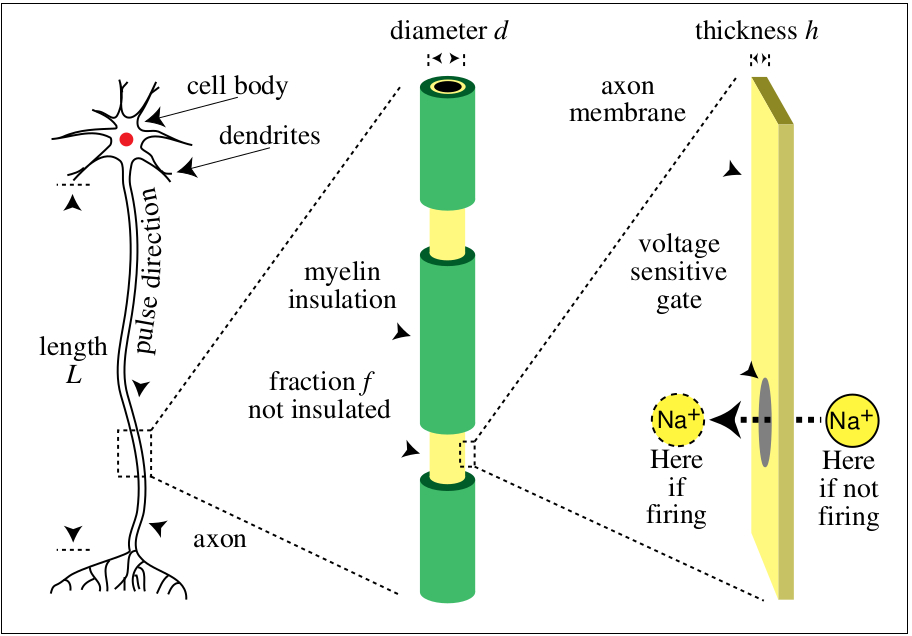
\includegraphics[scale=0.4]{graphics/neuron_schematic.jpg}
	\caption{Schematische Darstellung einer Nervenzelle. Hervorgehoben sind die Größen, die für die Abschätzung der 
		Anzahl der Na$^{+}$-Ionen verwendet werden, die sich in Superposition befinden.\cite{Tegmark_99} \label{fig:neuron}}
\end{figure}

Für die Abschätzung der Größenordnung der Dekohärenz-Zeitskala werden die drei am häufigsten auftretenden
Wechselwirkungen mit der Umgebung
betrachte. Dies sind zum einen Stöße der Na-Ionen mit anderen Ionen oder Wassermolekülen und zum anderen
Coulomb-Abstoßung zwischen den gleich geladenen Na-Ionen.
Die Zeitentwicklung des Zustandes $\rho$ lässt sich für diese drei Wechselwirkungen allgemein mit  
\begin{empheq}{align}
	\label{eq:time_evolution}
	\rho(r, r^{\prime},t_{0}+t) = \rho(r, r^{\prime},t_{0}) f(r,r^{\prime},t)
\end{empheq}
beschreiben wobei die Funktion $f(r,r^{\prime},t)$ von der Wechselwirkung 
und nicht von dem Zustand des Ions abhängt. Eine detailliert Betrachtung der Berechnungen
ist in \cite{Tegmark_99} zu finden. 
Als Dekohärenz-Zeitskalen für die drei betrachteten Wechselwirkungen ergeben sich die in 
\cref{tab:decoherence_time} dargestellten.
\begin{table}
	\centering
	\begin{tabular}{lc}
		\toprule
		Wechselwirkung & $\tau_{dec}$\\
		\midrule
		Stoß mit Ion & \SI{e-20}{s} \\ 
		Stoß mit H$_2$O & \SI{e-20}{s} \\ 
		Coulombabstoßung & \SI{e-19}{s} \\ 
		\bottomrule
	\end{tabular}
	\caption{Zeitskalen der Dekohärenz aufgrund der betrachteten Wechselwirkungen der Na$^{+}$-Ionen
		in Superposition. Abgewandelt aus: \cite{Tegmark_99} \label{tab:decoherence_time}}
\end{table}

Es zeigt sich als das Superpositionen von Neuronen, wie sie hier betrachtet wurde auf Zeitskalen der 
Größenordnung \SI{e-20}{s} zerstört werden. Verglichen mit den typischen Dynamik-Zeitskalen, die für 
die schnellsten Neuronen bei etwa \SI{e-3}{s} liegen, zeigt sich ein Unterschied von etwa 17 Größenordnungen.
Entsprechend kann gefolgert werden das Superpositionen zwischen unterschiedlichen Neuronenzuständen bereits 
bei der Entstehung unterdrückt werden und diese Gehirnprozesse somit klassisch beschrieben werden müssen. 
 
	\section{Bewusstsein als Aggregatzustand}
	% !TeX root = ../paper_observer_consciousness.tex

Die bekannten Aggregatzustände lassen sich durch die Unterschiede in ihren Eigenschaften einteilen,
so haben Festkörper eine quasi-unendliche Viskosität. Alle übrigen Stoffe zeigen weiter Unterschiede,
beispielsweise sind Flüssigkeiten weniger kompressible und Gase und Plasmen lassen sich durch ihr
Leitfähigkeit unterscheiden. 

In analoger Form lässt sich nun die Frage nach den Eigenschaften stellen, die Materie haben muss, 
die bewusst ist. Ähnliche Überlegungen wurden bereits angestellt, um festzustellen welche Eigenschaften 
\emph{computronium} haben muss, ein Zustand von Materie der \enquote{berechnen} kann.
Zwei mögliche Eigenschaften von bewusster Materie, Integrierte Information und Unabhängigkeit werden im 
folgenden erläutert.

		\subsection{Integrierte Information}
		% !TeX root = ../paper_observer_consciousness.tex

Integrierte Information als Maß für das Bewusstsein zu verwenden ist Teil der \emph{Integratet Information Theory}
des Neurowissenschaftlers Giulio Tononi.\,\cite{Tononi_08} 
Die im Folgenden verwendete formale Definition für die Integrierte Information $\Phi$ weicht dabei von der 
Definition nach Tononi ab, ermöglicht aber ähnliche Aussagen. Die Integriert Information entspricht 
hier der minimalen Transinformation $I(\rho)$ die durch eine Trennung des Zustands $\rho$ in zwei Teilsystem
Zustände $\rho_{1}$ und $\rho_{2}$ erreicht werden kann.

\begin{empheq}{equation}
	\Phi = I_{\mathrm{min}} = \min I(\rho) = \min \del{S(\rho_1) + S(\rho_2) - S(\rho)}
\end{empheq}
Da ein Zustand mit $\Phi = I = 0$ in vollkommen unabhängige Teilzustände zerlegt werden kann und 
demnach möglichst unabhängigen Teilzustände die geringste Transinformation haben,  
wurde die Trennung des Zustands $\rho$  zur Bestimmung der Integrierten Information von Tononi
als \Quote{the cruelest cut} bezeichnet.

Eine mögliche Veranschaulichung von Integrierten Information ist das Speichern von Information mit 
unter Verwendung von Redundanz oder Fehlerkorrektur-Mechanismen. Dies findet beispielsweise in 
den weit verbreiteten QR-Codes Anwendung, deren Informationen nach Verlust eines Teils des Musters immer
noch zugänglich sind. Ein Beispiel dafür ist in \cref{fig:qrcode} dargestellt.
Durch numerische Berechnung kann die maximal mögliche Integration von Information eines Systems mit einer
festen Größe  von $n$ bit bestimmt werden. In  \cref{fig:maximal_integrated_information} ist dies beispielhaft 
für $n = \SI{14}{bit}$ gezeigt. Es ergibt sich, dass die maximal mögliche Integration für die Auswahl von 
{$\large \sfrac{n}{2}$} bit  zum speichern der Information vorliegt. Die übrigen {$\large \sfrac{n}{2}$} bit sorgen 
entsprechend für die notwendige Redundanz.


\begin{figure}
	\centering
	
\includegraphics[scale=0.15]{graphics/qrcode_damaged.jpg}
	\caption{Beispielhafte Darstellung eines QR-Code, dessen Information auch nach Entfernen von etwa 
		\SI{30}{\percent} des Musters noch nicht gelöscht ist.\label{fig:neuronqrcode}}
\end{figure}  
\begin{figure}
	\centering
	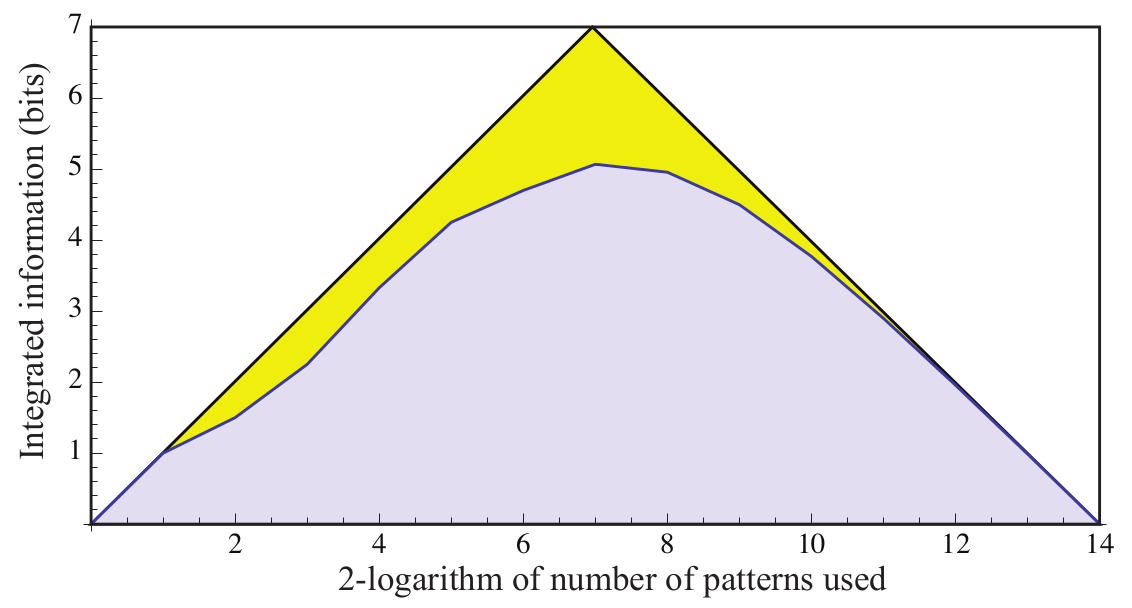
\includegraphics[scale=0.25]{graphics/integrated_information_graph.jpg}
	\caption{Darstellung der Ergebnisse der numerischen Suche nach maximaler Intgration in einem System 
		mit $n = \SI{14}{bit}$. Das Dreieck im Hintergrund stellt dabei die theoretisch maximal mögliche 
		Integration dar, die dem Minimum von Speicher-bits und Redundanz-bits entspricht. Die grau dargestellte
		Kurve gibt jeweils die maximale Integration für die jeweilige Anzahl an Speicher-bits an. \label{fig:maximal_integrated_information}}
\end{figure}  

\begin{figure}
	\centering
	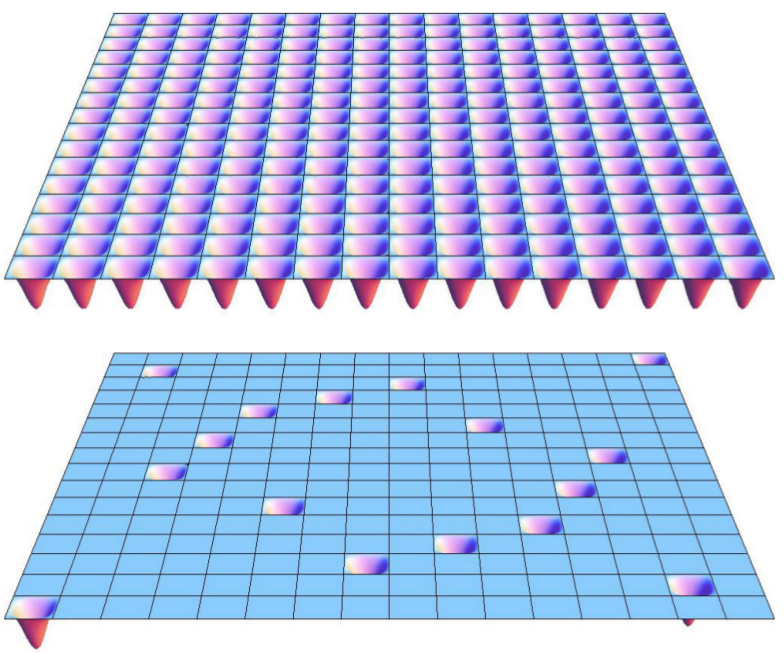
\includegraphics[scale=0.25]{graphics/egg_crate_potentials.jpg}
	\caption{Darstellung von zwei Eierkarton-Potentiallandschaften einmal mit 256 Minima (oben) und einmal 
		mit 16 Minima (unten). Ein Zustand im unteren System weißt eine gute Integration auf ein Zustand im oberen System ist gar nicht integriert.\label{fig:eggcrate_potential}}
\end{figure}  


Die Übertragung diese Konzepts in physikalische Systeme ist beispielsweise unter Betrachtung von 
\enquote{Eierkarton}-Potentiallandschaften, wie in \cref{fig:eggcrate_potential} dargestellt, möglich.
In dem Beispiel des dargestellten 16$\times$16-Gitters lässt sich die Position $\del{x,y}$ eines Potentialminimums
mit unter Verwendung von je einer 4-bit-Zahl ($0_2$ -- $15_2$) für $x$ und $y$ kodieren. Für die beiden dargestellten 
Potentiallandschaften ergeben sich für die Integrierte Information die Werte $\Phi_{\mathrm{oben}} = 0$  und 
$\Phi_{\mathrm{unten}} = 2$. Diese Unterschiede in der Integration lassen sich folgender Maßen veranschaulichen.
Kennt man für beide der Potentiale nur einer der beiden Positionen $x$ oder $y$ so gibt das ober Potential keinen
Aufschluss auf die andere Komponente während diese im unteren festzustellen ist.

Betrachtet man nun neben der Information in einem n-bit-Zustand für die nach Shannon in etwa $S(\rho) \sim \log_{2}(\text{\# möglicher Zustände}) \sim n$. Die Information, die in einem System mit $k$ Minima so ergibt 
sich $S(H) \sim \log_{2}(\text{\# möglicher } H) \sim kn$. 
Setzt man nun beispielhaft die Anzahl der Neuronen im menschlichen Gehirn an und maximiert die Integrierte
Information die in diesem System steckt, ergibt sich die dafür notwendige Information zu 
\begin{empheq}{equation}
	S(H) \sim \sqrt{2^{n}}\frac{n}{2} \sim 10^{10^{10}} \text{bit}.
\end{empheq}
Diese Anzahl übersteigt die Anzahl der Teilchen im Universum $\num{e89}$ um ein vielfaches. Die notwendige Dynamik 
für maximale Integration im Gehirn des Menschen ist entsprechen viel zu komplex um 
realisiert zu werden.

  





		\subsection{Unabhängigkeit}
		\begin{frame}{Unabhängigkeit}
	\begin{columns}
		\alt<1>{\begin{column}{0.55\textwidth}
			\begin{itemize}
				\item{Als Maß für Unabhängigkeit wiederum $\Phi$ verwendbar}
				\item{klassisches 2-bit-System, {\footnotesize$\rho = \begin{pmatrix} P(\downarrow\downarrow) & P(\downarrow\uparrow)\\P(\uparrow\downarrow) & P(\uparrow\uparrow)\end{pmatrix}$}}
				\begin{itemize}
					\item{nur ein Schnitt in zwei einzelne bits möglich $\Rightarrow \Phi = I$}
					\item{helles Dreieck}
				\end{itemize}
				\item{2-qbit-System: $\rho \in \mathbb{R}^{4\times4}$}
				\begin{itemize}
					\item{zusätzlich dunkles Dreieck}
					\item{$\Phi = \displaystyle\min_{U} I\del{U\rho U^{\dagger}}$}
				\end{itemize}
			\end{itemize}		
		\end{column}}{}
		\alt<2>{\begin{column}{0.55\textwidth}
				\begin{itemize}
					\item{Bell-Paar (4): $\ket{\Psi} = \frac{1}{\sqrt{2}} \del{\ketup\!\ketup + \ketdown\!\ketdown}$  }
					\begin{itemize}
						\item{Reiner Zustand,\\ Trafo $\Rightarrow$ $\rho = \ketup\!\braup$}
						\item{separabel $\Rightarrow \Phi = 0$}
					\end{itemize}
					\item{maximale Verschränkung, keine Integrierte Information}
					\begin{itemize}
						\item{\Quote{the \textbf{cruelest} cut}}
					\end{itemize}
				\end{itemize}		
			\end{column}}{}
		
		\begin{column}{0.55\textwidth}
			\centering
			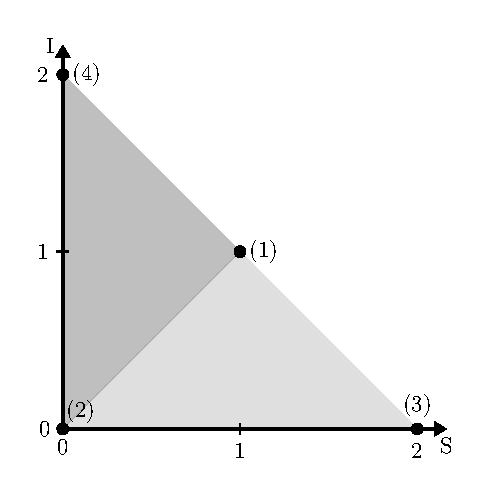
\includegraphics[scale=0.65]{graphics/presentation_qm.pdf}\,\cite{Tegmark_15_long}
			\footnotesize
			(1): $\rho = \frac{1}{2} \del{\ketup\!\braup + \ketdown\!\bradown}$\\
			\hspace{-1.65cm}(2): $\rho = \ketup\!\braup$\\
			\hspace{-.2cm}(3): $\rho = \frac{1}{4} (\ketup\!\braup + \ketdown\!\braup$\\\qquad\qquad $+ \ketup\!\bradown + \ketdown\!\bradown)$\\
			(4): $\rho = \frac{1}{2} \del{\ketup\!\ketup + \ketdown\!\ketdown}$ \\\qquad\qquad$\del{\braup\!\braup + \bradown\!\bradown} $\\
		\end{column}		
	\end{columns}
\end{frame}
		%\subsection{Dynamik und Autonomie}
		%% !TeX root = ../paper_observer_consciousness.tex
	\section{Schlussbetrachtung}
	% !TeX root = ../paper_observer_consciousness.tex
	\newpage
	\nocite{Zeh_00}
	\printbibliography
\end{document}